\section{VC Dimensions}
\label{sec:vc-dimension}
\begin{enumerate}
\item ~[10 points] Suppose you have a finite hypothesis space
  $\mathcal{C}$. Show that its VC dimension at most
  $\log_2|\mathcal{C}|$ (Hint: You also prove this by contradiction.)

The growth function $m_\mathcal{C}(N)$ for a hypothesis class $\mathcal{C}$ is defined as the maximum number of dichotomies than can be generated by $\mathcal{C}$ on any $N$ points. 

The VC dimension of $\mathcal{C}$,$d_{VC}(\mathcal{C})$, is the largest $N$ for which $m_\mathcal{C}(N)=2^N$. In other words, $d_{VC}(\mathcal{C})$ is the largest $N$ that can be split into all possible dichotomies by the hypothesis class $\mathcal{C}$.

Each hypothesis in the hypothesis class $\mathcal{C}$ can at the maximum generate a distinct dichotomy. That means, there could be a maximum of $\left | \mathcal{C} \right| $ dichotomies that can be generated by the hypothesis class $\mathcal{C}$.

This means that $d_{VC}(\mathcal{C})$ is the largest $N$ such that 

\begin{equation*}
\begin{aligned}
m_\mathcal{C}(N)=2^N &\leq \left | \mathcal{C} \right| \\
N \log_2 2 &\leq \log_2 \left | \mathcal{C} \right| \\
N &\leq \log_2|\mathcal{C}|
\end{aligned}
\end{equation*}

This means that the VC dimension at most $\log_2|\mathcal{C}|$

\item ~[10 points] Given some finite domain set, $\mathcal{X}$, and a
  number $k \leq |\mathcal{X}|$, figure out the VC-dimension of each
  of the following classes and prove your claims:

  \begin{enumerate}
  \item
    $\mathcal{H}_{=k}^{\mathcal{X}} = \{h \in \{0,1\}^\mathcal{X} :
    |\{x : h(x) = 1\} | = k \}$. That is , the set of all functions that
    assign the value 1 to exactly $k$ elements of $\mathcal{X}$.

$d_{VC}(\mathcal{H})$, the VC dimension of the hypothesis class $\mathcal{H}$, is defined as the largest $N$ for which $m_{\mathcal{H}}(N) = 2^N$. The definition of $m_{\mathcal{H}} $ is similar to the one given above.\\

For the case of maximum number of dichotomies, we can consider that each hypothesis in $\mathcal{H}$ creates a distinct dichotomy. To find $d_{VC}(\mathcal{H})$ corresponding to this case, since we know that at exactly $k$ elements are assigned a label $1$ and the remaining elements are assigned label $0$, for the case of the VC dimension, the maximum number of dichotomies must be a power of $2$. Consider a subset of elements of $\mathcal{X}$, where $k$ elements are assigned label $1$ and $y$ elements are assigned label $0$.

\begin{equation*}
\begin{aligned}
\left | \mathcal{H} \right | &= 2^{k + y}\\
\log_2 \left | \mathcal{H} \right | &= k+y\\
y &= \log_2 \left | \mathcal{H} \right | - k\\
\end{aligned}
\end{equation*}

Since $d_{VC}(\mathcal{H})$, the VC dimension of the hypothesis class $\mathcal{H}$, is defined as the largest $N$ for which $m_{\mathcal{H}}(N) = 2^N$

\begin{equation*}
\begin{aligned}
2^{d_{VC}(\mathcal{H})} &= 2^{k+y}\\
&= 2^{k+\log_2 \left | \mathcal{H} \right | - k}\\
&= 2^{log_2 \left | \mathcal{H} \right |}\\
\implies d_{VC}(\mathcal{H}) &= \log_2 \left | \mathcal{H} \right |
\end{aligned}
\end{equation*}

  \item  $\mathcal{H}_{\leq k}^{\mathcal{X}} = \{h \in
    \{0,1\}^\mathcal{X} : |\{x : h(x) = 1\} | \leq k \quad or \quad |\{x
      : h(x) = 0\} | \leq k\}$. That is , the set of all functions that
    assign the value 1 or 0 to at most $k$ elements of $\mathcal{X}$.

For the case of a set of $d_{VC}(\mathcal{H})$ elements in $\mathcal{X}$, the label will be $1$ for between $0$ and $k$ elements. If this happens, there will be correspondingly between $k$ and $0$ elements with label $0$. So the total number of dichotomies will be
$$
\sum_{i=0}^k {N \choose i}
$$
where N is the number of elements chosen from $\mathcal{X}$.

Let $d_{VC}(\mathcal{H}) = y$. This means that

\begin{equation*}
\begin{aligned}
2^y &= \sum_{i=0}^k {N \choose i}\\
\implies d_{VC}(\mathcal{H}) &= y\\
 &= \log_2 \sum_{i=0}^k {N \choose i}
\end{aligned}
\end{equation*}

  \end{enumerate}

\item ~[10 points] Suppose we have an instance space consisting of
  real numbers and a hypothesis space $\mathcal{H}$ consisting of {\em
    two} disjoint intervals, defined by $[a, b]$ and $[c, d]$. That
  is, a point $x \in \Re$ is labeled as positive if, and only if,
  either $a \leq x \leq b$ or $c \leq x \leq d$. Determine the VC
  dimension of $\mathcal{H}$?

Since the two intervals are disjoint, there are five regions in the instance space that are defined by the intervals:

\begin{enumerate}
\item before the first interval
\item inside the first interval
\item between the first and second intervals
\item inside the second interval
\item after the second interval
\end{enumerate}

So the maximum number of points that can possibly be split into all possible dichotomies is $5$. If the $5$ points can be split into all possible dichotomies then the dichotomy $\{1,0,1,0,1\}$ should be one of them (I am representing a positive label by $1$ and a negative label by $0$). However, this dichotomy is not possible since there are only two intervals where the label can be $1$ and the label $\{1,0,1,0,1\}$ requires three such intervals.

Consider $4$ points. These $4$ points can be split into the dichotomies $\{\{0,0,0,0\},\{0,0,0,1\},\\\{0,0,1,0\},\{0,0,1,1\},\{0,1,0,0\},\{0,1,0,1\},\{0,1,1,0\},\{0,1,1,1\},\{1,0,0,0\},\{1,0,0,1\},\\\{1,0,1,0\},\{1,0,1,1\},\{1,1,0,0\},\{1,1,0,1\},\{1,1,1,0\},\{1,1,1,1\}\}$. These are all possible dichotomies that can be generated using $4$ points and the hypothesis space $\mathcal{H}$.\\ 

So $d_{VC}(\mathcal{H}) = 4$.

\item ~[15 points] We have a learning problem where each example is a
  point in $\Re^2$. The concept class $H$ is defined as follows: A
  function $h \in H$ is specified by two parameters $a$ and $b$. An
  example ${\bf x} = \{x_1, x_2\}$ in $\Re^2$ is labeled as $+$ if and
  only if $x_1 + x_2 \geq a$ and $x_1 - x_2 \leq b$ and is labeled $-1$
  otherwise.

  For example, if we set $a = 0, b = 0$, the grey region in figure
  \ref{f1} is the region of ${\bf x} = \{x_1, x_2\}$ that has label
  $+1$.

  \begin{figure}[h!]
    \centering
    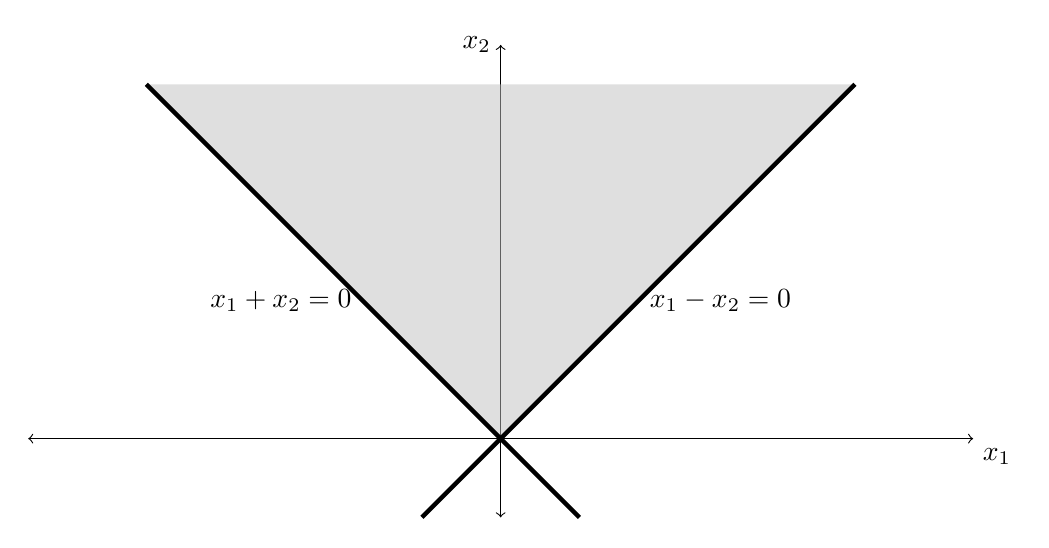
\begin{tikzpicture}[domain=0:2]
      \draw[<->] (-6,0) -- (6,0) node[below right] {$x_1$};
      \draw[<->] (0,-1) -- (0,5) node[left] {$x_2$};
      \fill[gray!50,opacity=0.5] (0,0) -- (4.5,4.5) -- (-4.5,4.5) -- (0,0);
      \draw [ultra thick] (4.5,4.5) -- node [midway,right] {$x_1 -x_2 = 0$} (-1,-1);
      \draw [ultra thick] (-4.5,4.5) --  node [midway,left] {$x_1 + x_2 = 0$}(1,-1);
    \end{tikzpicture}
    \caption{An example with $a = 0, b = 0$. All points in the gray region
      (extending infinitely) shows the region that will be labeled as
      positive.} \label{f1}
  \end{figure}



  What is the VC dimension of this class?

The concept class contains individual hypothesis' that consist on two arms that can intersect anywhere on $\Re^2$ and can cover an infinite arc from any angle from $0\si{\degree}$ to $360\si{\degree}$. Consider the case of three collinear points which have labels $\{+1, -1, +1\}$. This classification clearly cannot be satisfied by any of the hypothesis in the hypothesis class. Any two points ($2^1$ points) with any distribution of $+1$ and $-1$ can be covered.\\

So $d_{VC}(H) = 1$.

\item ~[{\bf For 6350 Students,} 15 points] Let two hypothesis classes
  $H_1$ and $H_2$ satisfy $H_1 \subseteq H_2$. Prove: $VC(H_1) \leq
  VC(H_2)$.

Consider any set of points $N$ that are labelled by $H_2$. The same set of points may not result in the same number of dichotomies by $H_1$ as those produced by $H_2$. The reason is that $H_2$ may have hypotheses that are not present in $H_1$, whereas all hypotheses in $H_1$ will be present in $H_2$. This means that $H_2$ can be more expressive than $H_1$. This means that $d_{VC}(H_1) \leq d_{VC}(H_2)$.

\end{enumerate}
%%% Local Variables:
%%% mode: latex
%%% TeX-master: "hw"
%%% End:
